
%% Commands for TeXCount
%TC:macro \cite [option:text,text]
%TC:macro \citep [option:text,text]
%TC:macro \citet [option:text,text]
%TC:envir table 0 1
%TC:envir table* 0 1
%TC:envir tabular [ignore] word
%TC:envir displaymath 0 word
%TC:envir math 0 word
%TC:envir comment 0 0
%%

%%
\PassOptionsToPackage{prologue}{xcolor}
\documentclass[manuscript,screen,review]{acmart}
%%
% Este bloque define el comando \BibTeX para escribir "BibTeX" con el formato correcto.
\AtBeginDocument{%
  \providecommand\BibTeX{{%
    Bib\TeX}}}
% Comandos para establecer derechos de autor y metadatos de publicación ACM:
% - \setcopyright{acmlicensed}  % Tipo de licencia (consultar el valor correcto con ACM)
% - \copyrightyear{2018}        % Año de copyright (año de publicación)
% - \acmYear{2018}              % Año de la conferencia o revista ACM
% - \acmDOI{XXXXXXX.XXXXXXX}    % DOI oficial del artículo (asignado por ACM)
% Estos comandos deben incluirse en artículos originales para ACM (conferencia o revista).
% Sirven para establecer metadatos de publicación y derechos de autor desde el primer envío.
\acmConference[Conference acronym 'XX]{Make sure to enter the correct
  conference title from your rights confirmation email}{June 03--05,
  2018}{Woodstock, NY}
%%
%%  Uncomment \acmBooktitle if the title of the proceedings is different
%%  from ``Proceedings of ...''!
%%
%%\acmBooktitle{Woodstock '18: ACM Symposium on Neural Gaze Detection,
%%  June 03--05, 2018, Woodstock, NY}
\acmISBN{978-1-4503-XXXX-X/2018/06}

\captionsetup{hypcap=false}
\setlength{\headheight}{21pt}
%%
%% ID de envío.
%% Usa este comando cuando envíes un artículo a un evento patrocinado.
%% Recibirás un ID único de envío por parte de los organizadores
%% del evento, y este ID debe usarse como parámetro en este comando.
%%\acmSubmissionID{123-A56-BU3}

%%
%% Para gestionar citas y bibliografía, se recomienda usar archivos
%% de bibliografía en formato BibTeX.
%%
%% Puedes usar BibTeX con el estilo ACM-Reference-Format,
%% o BibLaTeX con los estilos acmnumeric o acmauthoryear,
%% que incluyen soporte avanzado para citar software mediante
%% el paquete biblatex-software, también disponible por separado en CTAN.
%%
%% Consulta los archivos sample-*-biblatex.tex como plantillas que muestran
%% los estilos biblatex.
%%

%%
%% La mayoría de publicaciones de ACM usan citas y referencias numeradas.
%% El comando \citestyle{authoryear} cambia al estilo "autor-año".
%%
%% Si preparas contenido para un evento patrocinado por ACM SIGGRAPH,
%% debes usar el estilo "autor-año" para las citas y referencias.
%% Si descomentas el siguiente comando, activarás ese estilo.
%%\citestyle{acmauthoryear}


%%
%% end of the preamble, start of the body of the document source.
\begin{document}
\setcopyright{none}
%% El comando "title" tiene un parámetro opcional,
%% que permite definir un "título corto" para los encabezados de página.
\title{Tratamiento térmico de beterraga (Beta vulgaris) y calidad sensorial-fisicoquímica de chocotejas con quinua y kiwicha pop.}
%%
%% Los comandos "author" y relacionados definen los autores y sus afiliaciones.
%% Se destaca la afiliación compartida de los dos primeros autores y el uso de
%% "authornote" y "authornotemark" para indicar contribución compartida.
\author{David Helcias Espino Curi}
\orcid{0000-0002-1234-5678}
\email{david.espino.19@unsch.edu.pe}
\affiliation{%
  \institution{Universidad Nacional San Cristóbal de Huamanga}
  \city{Ayacucho}
  \country{Perú}
}
\author{Katherine Gloria Delgado Rojas}
\affiliation{%
  \institution{Universidad Nacional San Cristóbal de Huamanga}
  \city{Ayacucho}
  \country{Perú}
}
\author{Luis Enrique Pomahuacre Amao}
\affiliation{%
  \institution{Universidad Nacional San Cristóbal de Huamanga}
  \city{Ayacucho}
  \country{Perú}
}
\author{Stephany Tinco De la Cruz}
\affiliation{%
  \institution{Universidad Nacional San Cristóbal de Huamanga}
  \city{Ayacucho}
  \country{Perú}
}
\author{Ruth Cynthia Huaman Bonifacio}
\affiliation{%
  \institution{Universidad Nacional San Cristóbal de Huamanga}
  \city{Ayacucho}
  \country{Perú}
}
\author{Agustin Pauca Carhuas}
\affiliation{%
  \institution{Universidad Nacional San Cristóbal de Huamanga}
  \city{Ayacucho}
  \country{Perú}
}
\author{Rommel Aldo Rojas Pariona}
\affiliation{%
  \institution{Universidad Nacional San Cristóbal de Huamanga}
  \city{Ayacucho}
  \country{Perú}
}
\author{Edith Susan Pillaca Medina}
\affiliation{%
  \institution{Universidad Nacional San Cristóbal de Huamanga}
  \city{Ayacucho}
  \country{Perú}
}
%%
%% Por defecto, la lista completa de autores aparece en los encabezados de página.
%% Si la lista es muy larga y ocupa demasiado espacio, este comando permite
%% definir una versión abreviada para los encabezados.
\renewcommand{\shortauthors}{Espino Curi et al.}
%%
%% El resumen (abstract) es una síntesis breve del trabajo presentado en el artículo.
\begin{abstract}
    Este estudio evaluó el efecto del tratamiento térmico de la beterraga (\textit{Beta vulgaris} L.) sobre propiedades fisicoquímicas y sensoriales de chocotejas funcionales elaboradas con quinua y kiwicha \textit{pop}. Se aplicó un diseño completamente al azar con tres tiempos de cocción: 0, 20 y 40 minutos. Las muestras se caracterizaron en contenido de humedad, actividad de agua (\textit{a\textsubscript{w}}), pH, densidad y atributos sensoriales mediante una escala hedónica de 9 puntos. La humedad disminuyó significativamente con el tiempo de cocción (31,6\% en crudo a 26,6\% tras 40 min; p<0,05), al igual que la actividad de agua (0,84 a 0,75). La densidad aparente fue máxima en el tratamiento intermedio (955 kg/m\textsuperscript{3}), asociada a una textura más crujiente. El pH se mantuvo estable en todos los tratamientos. Sensorialmente, la cocción de 20 minutos obtuvo la mayor aceptabilidad global (8,1 puntos), destacando por textura crocante y sabor equilibrado. En cambio, la muestra cruda presentó exceso de humedad, mientras que la cocida 40 minutos mostró notas terrosas menos apreciadas. Se concluye que la cocción intermedia optimiza la calidad tecnológica y sensorial de las chocotejas, permitiendo prescindir de secados adicionales y facilitando el desarrollo de productos con etiqueta limpia y uso de ingredientes andinos de alto valor nutricional. Futuras investigaciones deberían evaluar la estabilidad de compuestos bioactivos y la vida útil comercial.
\end{abstract}
%%
%% El siguiente bloque fue generado en base a los conceptos ACM más cercanos al área de Ciencia y Tecnología de Alimentos y Productos Funcionales.
%%
%-------------------------------------------------------
% Clasificación CCS (versión adaptada en español)
%-------------------------------------------------------
\begin{CCSXML}
<ccs2012>
  <concept>
    <concept_id>10010405.10010469.10010470</concept_id>
    <concept_desc>Ingenier\'{i}a de alimentos~Ciencia y tecnolog\'{i}a de alimentos</concept_desc>
    <concept_significance>500</concept_significance>
  </concept>
  <concept>
    <concept_id>10010147.10010341.10010349.10010350</concept_id>
    <concept_desc>Matem\'aticas aplicadas~Dise\~{n}o experimental</concept_desc>
    <concept_significance>300</concept_significance>
  </concept>
  <concept>
    <concept_id>10010405.10010444.10010449</concept_id>
    <concept_desc>Ingenier\'{i}a de alimentos~Productos de confiter\'ia</concept_desc>
    <concept_significance>100</concept_significance>
  </concept>
</ccs2012>
\end{CCSXML}

\ccsdesc[500]{Ingenier\'{i}a de alimentos~Ciencia y tecnolog\'{i}a de alimentos}
\ccsdesc[300]{Matem\'aticas aplicadas~Dise\~{n}o experimental}
\ccsdesc[100]{Ingenier\'{i}a de alimentos~Productos de confiter\'ia}

%-------------------------------------------------------
% Palabras clave (versión en español)
%-------------------------------------------------------
\keywords{chocotejas, beterraga, quinua pop, kiwicha pop, an\'alisis sensorial, textura, humedad, densidad, actividad de agua}

%%-------------------------------------------------------
%% Fechas de procesamiento del manuscrito (en español)
%%-------------------------------------------------------
\received{03 de julio de 2025}          % Fecha de recepción
\received[revisado]{\textit{pendiente}} % Fecha de revisión (rellenar cuando proceda)
\received[aceptado]{\textit{pendiente}} % Fecha de aceptación (rellenar cuando proceda)

\maketitle
%%
\section{Introducción}

    La remolacha o beterraga (\textit{Beta vulgaris} L.) constituye una raíz de notable interés en la industria alimentaria y en la investigación nutracéutica debido a su elevado contenido de compuestos bioactivos como betalainas, nitratos y polifenoles, los cuales han sido asociados con beneficios cardiovasculares, antioxidantes y antiinflamatorios \cite{Clifford2021,Siervo2016,WoottonBeard2011}. Entre estos compuestos, las betalainas no sólo confieren el característico color rojo intenso, sino que también actúan como potentes agentes antioxidantes con aplicaciones potenciales como colorantes naturales y componentes especializados en productos alimenticios \cite{Neelwarne2013,Montoya2011}. Estudios recientes han documentado que la aplicación de tratamientos térmicos a la remolacha puede inducir pérdidas parciales de estos pigmentos, modificar la actividad antioxidante y alterar parámetros tecnológicos críticos como la humedad y la textura, dependiendo de la duración y temperatura del proceso \cite{ArrudaRamos2017,Montoya2011}.
    
    Por otro lado, los pseudocereales andinos quinua (\textit{Chenopodium quinoa}) y kiwicha (\textit{Amaranthus spp.}) se han consolidado como ingredientes estratégicos en el desarrollo de alimentos innovadores, dada su composición nutricional que combina proteínas de alto valor biológico, fibra dietaria, vitaminas y minerales \cite{RepoCarrascoValencia2009,Singh2023}. La incorporación de estos pseudocereales en su forma expandida (\textit{pop}) en matrices de confitería permite mejorar la textura y reducir la densidad aparente, contribuyendo a la diferenciación sensorial y a la percepción de valor agregado en los consumidores. No obstante, la literatura disponible se ha centrado principalmente en estudios composicionales o en aplicaciones independientes de cada ingrediente, por lo que persisten vacíos relevantes sobre la influencia combinada del tiempo de cocción de la beterraga en la calidad fisicoquímica y sensorial de productos que integren estos pseudocereales.
    
    El presente estudio se planteó con el propósito de evaluar el efecto de tres tiempos de cocción (0, 20 y 40 minutos) de la beterraga sobre propiedades fisicoquímicas (humedad, actividad de agua, pH, densidad) y sensoriales (apariencia, aroma, sabor, textura y aceptabilidad global) de chocotejas especializadas elaboradas con quinua y kiwicha \textit{pop}. Este enfoque busca aportar evidencia que contribuya a optimizar el desarrollo de confitería diferenciada con ingredientes naturales, atendiendo simultáneamente la calidad tecnológica y la percepción del consumidor.
    %=========================================================
\section{Materiales y Métodos}
    %=========================================================

    \subsection{Materia prima y suministros}
    Se emplearon raíces frescas de beterraga (\textit{Beta vulgaris} L.) adquiridas en el mercado principal de Ayacucho (Perú).  
    La cobertura se formuló con chocolate \emph{bitter} al 55\,\% de cacao de marca comercial.  
    Como agentes de crocancia se utilizaron quinua \emph{pop} y kiwicha \emph{pop} suministradas por proveedores locales certificados.  
    Todos los insumos se almacenaron a (22–25)\,°C y 50–60\,\% de humedad relativa hasta su procesamiento.
        \begin{figure}[H]
          \centering
          \begin{minipage}{0.48\linewidth}
            \centering
            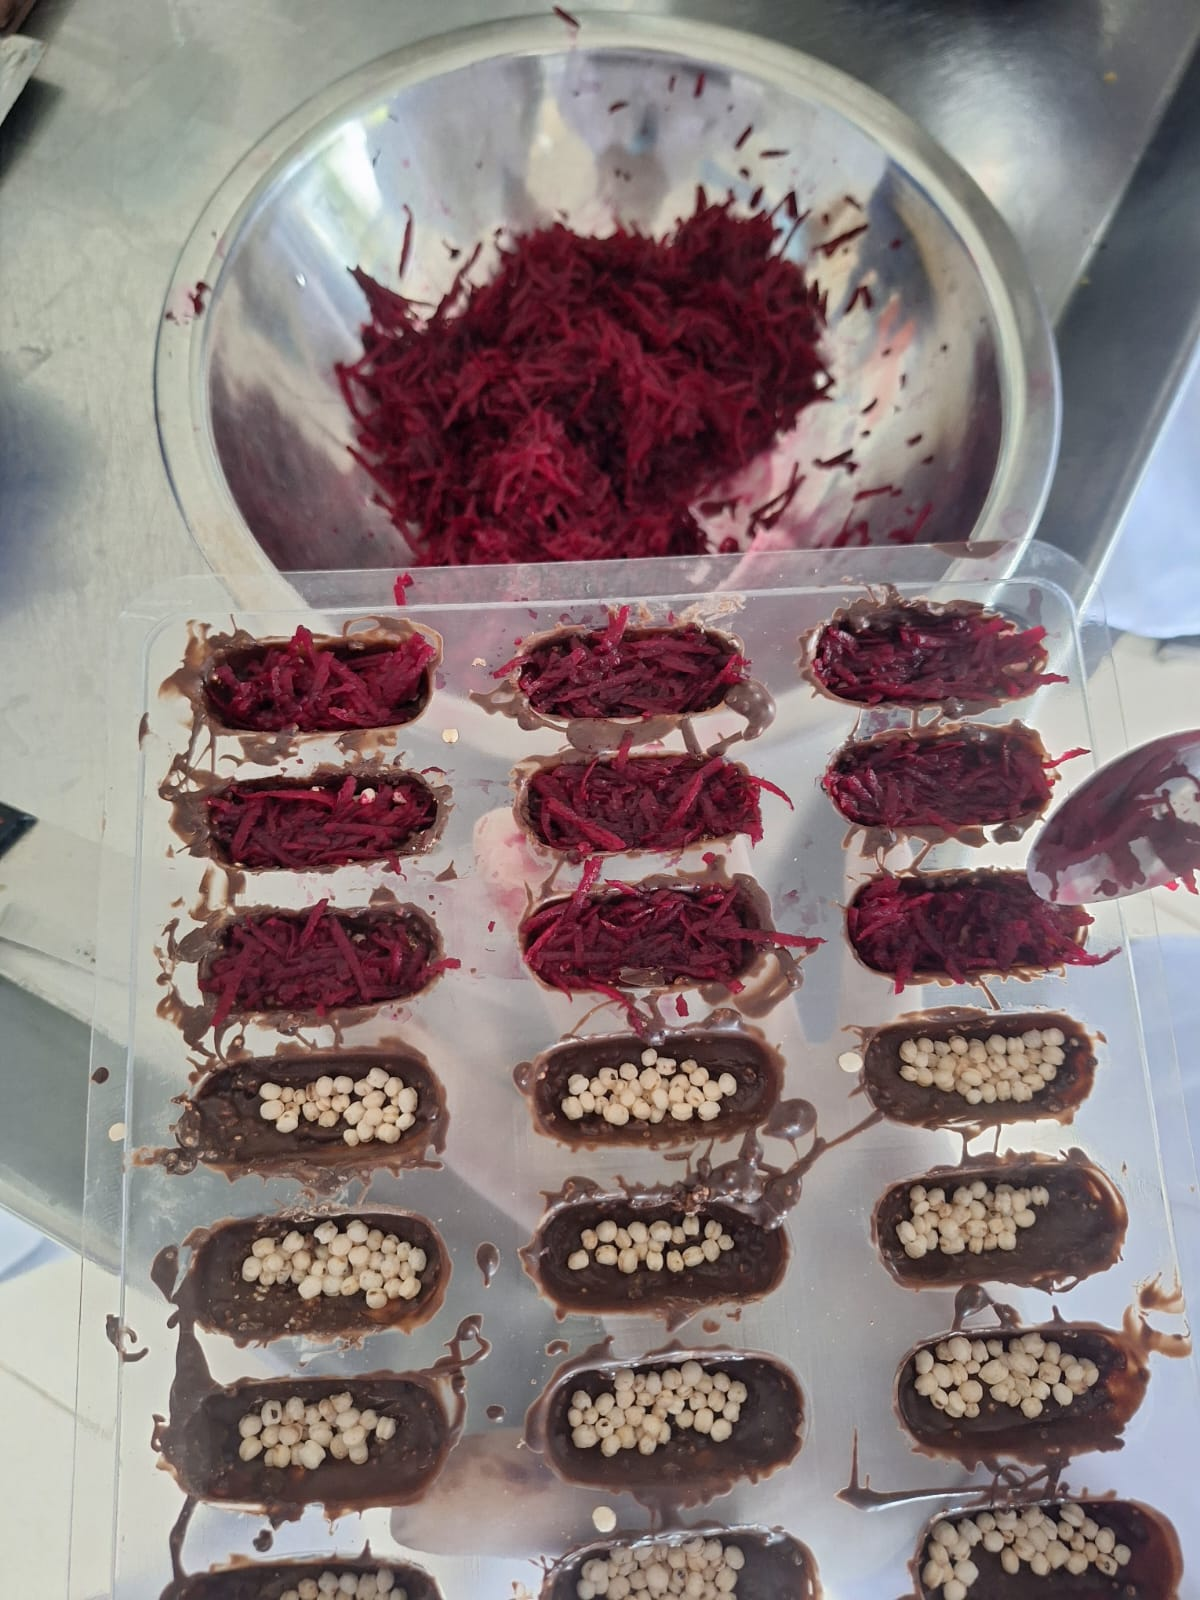
\includegraphics[width=0.9\linewidth]{imagen/beterraga-quinua.jpeg}
            \Description{Relleno de beterraga rallada con quinua pop en moldes}
            
            
            \small (a) Relleno de beterraga rallada dispuesto en moldes de chocotejas. Se observa la mezcla de quinua pop en la parte inferior.
          \end{minipage}
          \hspace{1em}
          \begin{minipage}{0.48\linewidth}
            \centering
            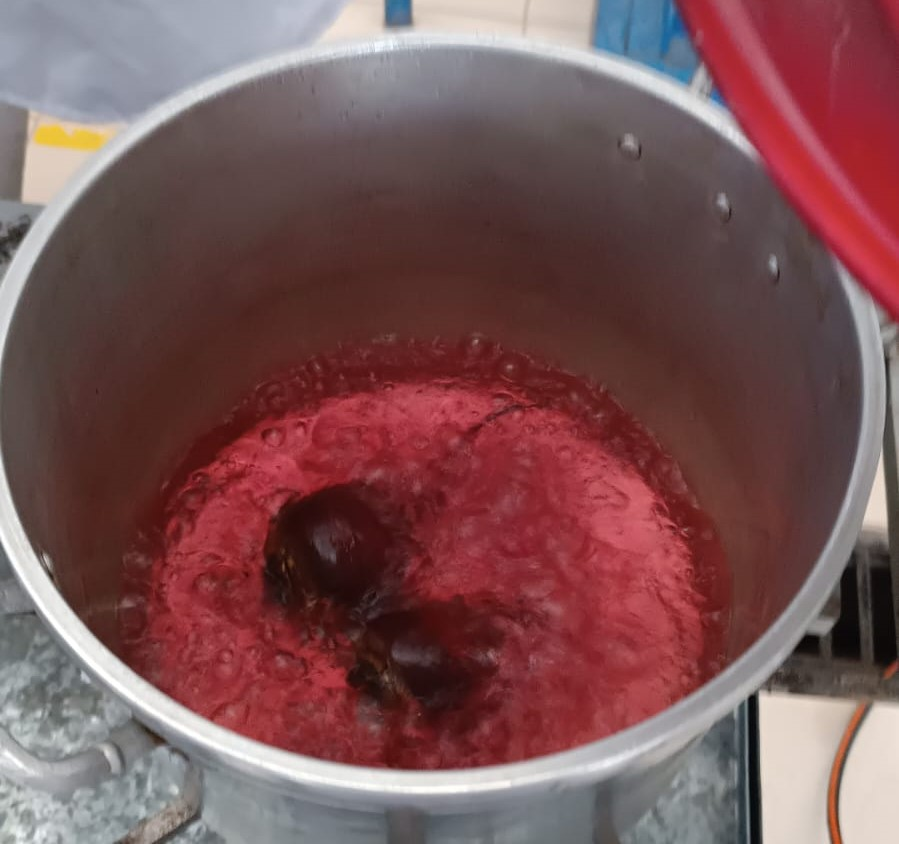
\includegraphics[width=0.9\linewidth]{imagen/coc-beterraga.jpeg}
            \Description{Cocción de beterraga entera en agua}
            
            
            \small (b) Cocción de beterraga entera en agua hirviendo durante los tratamientos térmicos.
          \end{minipage}
          
          \vspace{1ex}
          
          \begin{minipage}{0.48\linewidth}
            \centering
            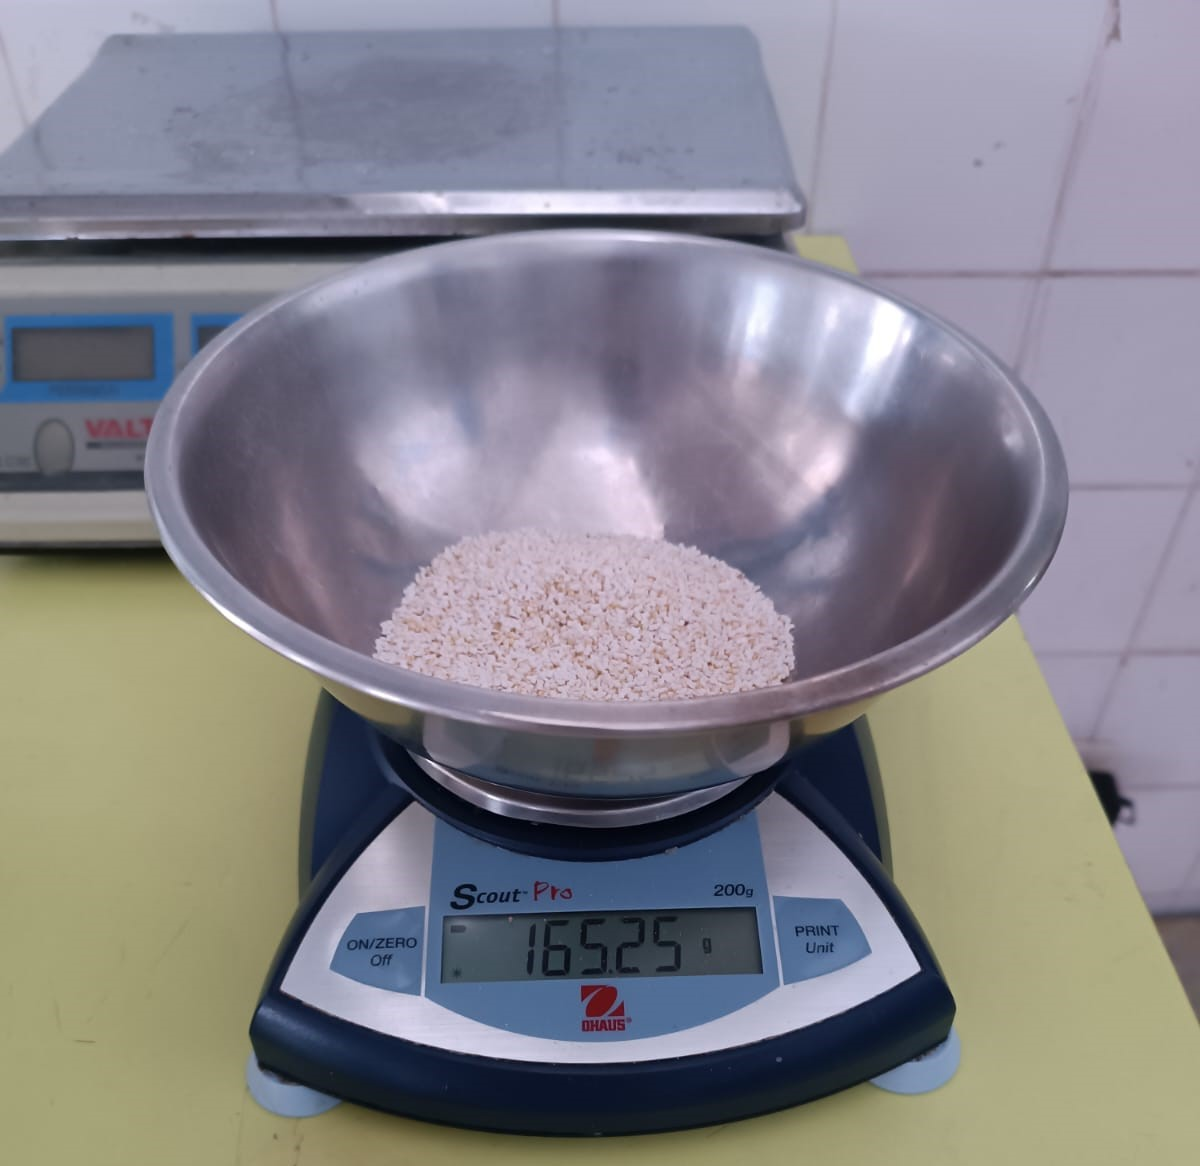
\includegraphics[width=0.9\linewidth]{imagen/kiwicha.jpeg}
            \Description{Pesaje de quinua pop en balanza}
            
            
            \small (c) Pesaje de quinua pop en balanza digital (165.25 g).
          \end{minipage}
          \hspace{1em}
          \begin{minipage}{0.48\linewidth}
            \centering
            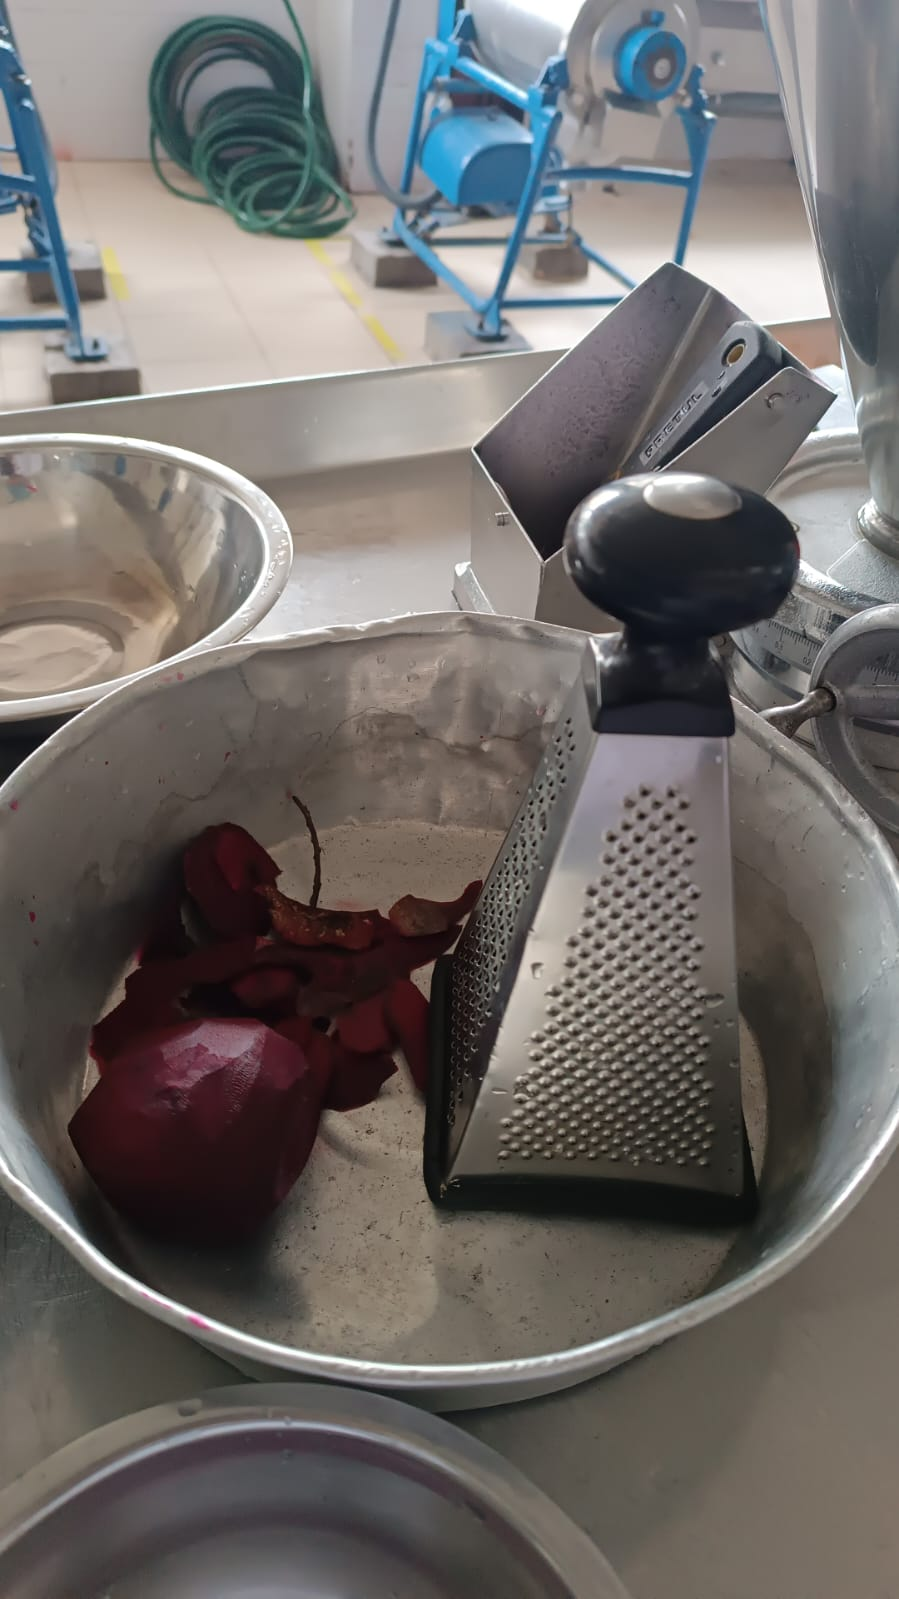
\includegraphics[width=0.9\linewidth]{imagen/rallado.jpeg}
            \Description{Rallado manual de beterraga cocida}
            
            
            \small (d) Rallado manual de beterraga cocida previo al mezclado con pseudocereales.
          \end{minipage}
          
          \caption{Etapas del proceso experimental de elaboración de chocotejas funcionales: tratamiento térmico, preparación del relleno y montaje en moldes con quinua y kiwicha pop.}
          \label{fig:proceso_chocotejas}
        \end{figure}

           
    \subsection{Disen~{n}o experimental}
    Se adoptó un diseño completamente al azar con tres tratamientos definidos por el tiempo de cocción de la beterraga:  
    T\textsubscript{0} (0 min, cruda),  
    T\textsubscript{1} (20 min) y  
    T\textsubscript{2} (40 min).  
    Cada tratamiento se elaboró en un lote de 24 chocotejas; mediante muestreo aleatorio se seleccionaron cuatro unidades por lote para los an\'alisis fisicoquímicos y sensoriales.
    
    \subsection{Procedimiento de elaboración}
    \paragraph{Cobertura.} El chocolate se fundió a 45\,°C, se atemperó a 27\,°C y finalmente se estabilizó a 31\,°C antes de mezclarse con kiwicha \emph{pop}.  
    La mezcla se vertió en moldes, se vibró para eliminar burbujas y se pre-enfrió a 12\,°C.
    
    \paragraph{Relleno.} La beterraga se lavó, desinfectó (100 mg·L\(^{-1}\) de NaClO, 5 min) y se sometió al tiempo de cocción correspondiente. Tras enfriamiento rápido (agua a 4\,°C, 5 min), las raíces se rallaron (2 mm) y se dejo oreando durante 1 h. Finalmente se mezclaron con quinua \emph{pop} (80:20, p/p) y se encapsularon dentro de la cobertura de chocolate.

                    El proceso se desarrolló según el siguiente flujograma para chocotejas:
                    
                    \begin{center}
                    \begin{minipage}{0.48\textwidth}
                    \centering
                    \begin{tikzpicture}[node distance=1.5cm]
                        % Cobertura de chocolate
                        \node (start) [process] {Recepción y selección de materia prima};
                        \node (fundido) [process, below of=start] {Fundido y atemperado del chocolate (45 °C, luego 27 °C y 31 °C)};
                        \node (mezcla) [process, below of=fundido] {Mezclado con kiwicha pop};
                        \node (moldeado) [process, below of=mezcla] {Moldeado y vibrado};
                        \node (enfriado) [process, below of=moldeado] {Pre-enfriamiento (12 °C) y desmoldado};
                        \draw [arrow] (start) -- (fundido);
                        \draw [arrow] (fundido) -- (mezcla);
                        \draw [arrow] (mezcla) -- (moldeado);
                        \draw [arrow] (moldeado) -- (enfriado);
                    \end{tikzpicture}
                    \captionof{figure}{Cobertura de chocolate}
                    \end{minipage}
                    \hfill
                    \begin{minipage}{0.48\textwidth}
                    \centering
                    \begin{tikzpicture}[node distance=1.5cm]
                        % Relleno
                        \node (start) [process] {Recepción y selección de materia prima};
                        \node (lavado) [process, below of=start] {Lavado y desinfección};
                        \node (coccion) [process, below of=lavado] {Tratamiento térmico: 0, 20 o 40 min};
                        \node (enfriado) [process, below of=coccion] {Enfriamiento rápido};
                        \node (rallado) [process, below of=enfriado] {Rallado longitudinal (2 mm)};
                        \node (deshidratado) [process, below of=rallado] {Oreado * 60 min};
                        \node (mezclado) [process, below of=deshidratado] {Mezclado con quinua pop};
                        \node (enrobado) [process, below of=mezclado] {Incorporación en la cobertura de chocolate};
                        \draw [arrow] (start) -- (lavado);
                        \draw [arrow] (lavado) -- (coccion);
                        \draw [arrow] (coccion) -- (enfriado);
                        \draw [arrow] (enfriado) -- (rallado);
                        \draw [arrow] (rallado) -- (deshidratado);
                        \draw [arrow] (deshidratado) -- (mezclado);
                        \draw [arrow] (mezclado) -- (enrobado);
                    \end{tikzpicture}
                    \captionof{figure}{Relleno}
                    \end{minipage}
                    \end{center}
        
    
    \subsection{Variables en estudio}
    \begin{itemize}
      \item \textbf{Variable independiente:} tiempo de cocción de la beterraga (0, 20 y 40 min).
      \item \textbf{Variables dependientes:} humedad (\%), actividad de agua (\textit{a\textsubscript{w}}), pH de cobertura y relleno, densidad aparente (kg·m\(^{-3}\)), y atributos sensoriales (apariencia, aroma, sabor, textura y aceptabilidad global).
    \end{itemize}
    
\subsection{Operacionalización de variables}
\begin{table}[htbp]
  \centering
  \caption{Operacionalización de las variables analizadas}
  \begin{tabular}{@{} llll @{}}
    \toprule
    \textbf{Variable} & \textbf{Indicador} & \textbf{Técnica} & \textbf{Unidad} \\
    \midrule
    Humedad           & Contenido de agua                    & Método gravimétrico en estufa, AOAC 925.10 (105 °C) & \% \\
    Actividad de agua & \textit{a\textsubscript{w}}          & Higrómetro AquaLab Serie 4TE, 25 °C, calibración NaCl & — \\
    pH (cobertura)    & pH                                   & Papel indicador de pH (intervalo 0–14, ±0.5 u.)      & — \\
    pH (relleno)      & pH                                   & Papel indicador de pH (intervalo 0–14, ±0.5 u.)      & — \\
    Densidad          & Masa / volumen                       & Balanza ±0.01 g; probeta graduada 100 mL (25 °C)      & kg·m\(^{-3}\) \\
    Aceptabilidad     & Puntuación hedónica                  & Escala de 9 puntos (1 = me disgusta ext., 9 = me gusta ext.) & puntos \\
    \bottomrule
  \end{tabular}
\end{table}

     \subsection{Análisis fisicoquímico}
    \begin{itemize}
      \item \textbf{Humedad}: secado en estufa a 105 °C hasta peso constante (AOAC 925.10).  
      \item \textbf{Actividad de agua}: higrómetro AquaLab 4TE (calibración estándar NaCl, \(a_\text{w}=0.75\)).  
      \item \textbf{pH}: suspensiones al 10 \% (m/v) medidas con potenciómetro Thermo Orion Star, calibrado a pH 4.00 y 7.00.  
      \item \textbf{Densidad aparente}: relación masa/volumen a 25 °C.  
    \end{itemize}
    
    \subsection{Evaluación sensorial}
    Veinte jueces no entrenados (18–35 años) calificaron las muestras, codificadas con números aleatorios, bajo luz neutra (5 500 K) y 22 °C. Se empleó una escala hedónica de 9 puntos (1 = ``me disgusta extremadamente''; 9 = ``me gusta extremadamente''). Los datos se recolectaron mediante formularios en línea.
    
    \subsection{Análisis estadístico}
    Las determinaciones fisicoquímicas se realizaron por triplicado. Se aplicó ANOVA de un factor; cuando se detectaron diferencias significativas (\(p<0.05\)) se utilizó la prueba de Tukey. El procesamiento se efectuó con SPSS v25 y se verificó la homogeneidad de varianzas (prueba de Levene).



%=========================================================
\section{Resultados}
%=========================================================

\subsection{Propiedades fisicoquímicas}

El contenido de humedad disminuyó significativamente ($p < 0.05$) con el aumento del tiempo de cocción (Tabla~\ref{tab:fisico}). La muestra sin cocción (T\textsubscript{0}) presentó un contenido de humedad de 31.6\,\%, mientras que T\textsubscript{1} (20 min) y T\textsubscript{2} (40 min) registraron valores de 27.2\,\% y 26.6\,\%, respectivamente. Este comportamiento coincide con lo reportado por Arruda Ramos \textit{et al.}~\cite{ArrudaRamos2017}, quienes atribuyen la reducción de humedad a la gelatinización parcial del almidón y la pérdida de agua libre durante la cocción.

\begin{figure}[H]
  \centering
  % ↓↓↓ 50 % del ancho del texto
  \resizebox{0.5\linewidth}{!}{%
    \begin{tikzpicture}
      \begin{axis}[
        width=\linewidth,      % reducción por resizebox
        ybar,
        bar width=18pt,
        ymin=0, ymax=35,
        ylabel={Humedad (\%)},
        symbolic x coords={T0,T1,T2},
        xtick=data,
        xticklabels={$T_{\mathrm{0}}$\\(0\,min),$T_{\mathrm{1}}$\\(20\,min),$T_{\mathrm{2}}$\\(40\,min)},
        nodes near coords,
        nodes near coords align={vertical},
        error bars/y explicit,
      ]
        % medias ± DE tomadas de la Tabla
        \addplot+[
          error bars/y explicit,
        ] coordinates {
          (T0,31.57) +- (0,0.48)
          (T1,27.16) +- (0,0.86)
          (T2,26.57) +- (0,1.09)
        };
      \end{axis}
    \end{tikzpicture}%
  }
  \caption{Contenido de humedad promedio ($\pm$ DE) según el tiempo de cocción de la beterraga.}
  \label{fig:humedad_bar}
\end{figure}


De igual modo, la actividad de agua ($a_w$) mostró un descenso progresivo de 0.84 (T\textsubscript{0}) a 0.77 (T\textsubscript{1}) y 0.75 (T\textsubscript{2}), implicando una mayor estabilidad microbiológica. La densidad aparente fue máxima en T\textsubscript{1} (955\,kg/m$^{3}$), lo que sugiere una estructura más compacta y favorable para la textura crujiente. Los valores de pH (tanto en cobertura como en relleno) no presentaron diferencias estadísticamente significativas ($p > 0.05$), manteniéndose dentro de los rangos recomendados para la estabilidad del producto.

\begin{table}[H]
  \centering
  \caption{Efecto del tiempo de cocción de la beterraga sobre las propiedades fisicoquímicas de las chocotejas (media $\pm$ DE, $n=4$).}
  \label{tab:fisico}
  \begin{tabular}{lccccc}
    \toprule
    \textbf{Tratamiento} & \textbf{Humedad (\%)} & $a_w$ & \textbf{Densidad (kg/m$^{3}$)} & \textbf{pH cobertura} & \textbf{pH relleno} \\
    \midrule
    T\textsubscript{0} (0 min)  & 31.57 $\pm$ 0.48\textsuperscript{a} & 0.84 $\pm$ 0.01\textsuperscript{a} & 934 $\pm$ 23\textsuperscript{b}  & 6.79 $\pm$ 0.03\textsuperscript{a} & 5.39 $\pm$ 0.03\textsuperscript{a} \\
    T\textsubscript{1} (20 min) & 27.16 $\pm$ 0.86\textsuperscript{b} & 0.77 $\pm$ 0.01\textsuperscript{b} & 955 $\pm$ 3\textsuperscript{a}   & 6.77 $\pm$ 0.02\textsuperscript{a} & 5.33 $\pm$ 0.02\textsuperscript{a} \\
    T\textsubscript{2} (40 min) & 26.57 $\pm$ 1.09\textsuperscript{b} & 0.75 $\pm$ 0.02\textsuperscript{b} & 949 $\pm$ 6\textsuperscript{a}   & 6.73 $\pm$ 0.01\textsuperscript{a} & 5.28 $\pm$ 0.01\textsuperscript{a} \\
    \bottomrule
  \end{tabular}
  \vspace{2mm}
  \begin{minipage}{0.9\linewidth}
  \footnotesize
  \textbf{Nota.} Letras distintas en una misma columna indican diferencias significativas entre medias según prueba de Tukey ($p<0.05$). Por ejemplo, valores con superíndice ``a'' difieren estadísticamente de los valores con ``b''.
  \end{minipage}
\end{table}




\subsection{Evaluación sensorial}

El an\'alisis sensorial (Tabla~\ref{tab:sensorial}) mostró que el tratamiento de 20 minutos (T\textsubscript{1}) obtuvo puntuaciones significativamente superiores ($p < 0.05$) en todos los atributos evaluados, alcanzando una aceptabilidad global de 8.1 $\pm$ 0.4 puntos. Los jueces describieron la textura como “muy crujiente” y el sabor equilibrado entre chocolate y beterraga. El exceso de humedad en T\textsubscript{0} disminuyó la crocancia, mientras que T\textsubscript{2} (40 min) presentó notas terrosas atribuidas a la degradación de pigmentos y formación de compuestos secundarios \cite{Montoya2011}.

\begin{table}[H]
  \centering
  \caption{Puntuaciones promedio ($n=20$, escala 1--9) de los atributos sensoriales de las chocotejas.}
  \label{tab:sensorial}
  \begin{tabular}{lccccc}
    \toprule
    \textbf{Tratamiento} & \textbf{Apariencia} & \textbf{Aroma} & \textbf{Sabor} & \textbf{Textura} & \textbf{Aceptabilidad global} \\
    \midrule
    T\textsubscript{0} (0 min)  & 6.2 $\pm$ 0.8\textsuperscript{b} & 6.0 $\pm$ 0.9\textsuperscript{b} & 6.1 $\pm$ 1.0\textsuperscript{b} & 6.3 $\pm$ 0.7\textsuperscript{b} & 6.0 $\pm$ 0.8\textsuperscript{b} \\
    T\textsubscript{1} (20 min) & 8.1 $\pm$ 0.5\textsuperscript{a} & 7.9 $\pm$ 0.6\textsuperscript{a} & 8.0 $\pm$ 0.4\textsuperscript{a} & 8.2 $\pm$ 0.5\textsuperscript{a} & 8.1 $\pm$ 0.4\textsuperscript{a} \\
    T\textsubscript{2} (40 min) & 7.0 $\pm$ 0.6\textsuperscript{b} & 6.8 $\pm$ 0.7\textsuperscript{b} & 6.9 $\pm$ 0.8\textsuperscript{b} & 7.1 $\pm$ 0.6\textsuperscript{b} & 7.0 $\pm$ 0.7\textsuperscript{b} \\
    \bottomrule
  \end{tabular}
  \vspace{2mm}
  \begin{minipage}{0.9\linewidth}
  \footnotesize
  \textbf{Nota.} Letras distintas en una misma fila indican diferencias significativas entre tratamientos según prueba de Tukey ($p<0.05$). Superíndices idénticos representan ausencia de diferencia estadística.
  \end{minipage}
\end{table}


\begin{figure}[H]
  \centering
  % Primera fila
  \begin{minipage}{0.3\linewidth}
    \centering
    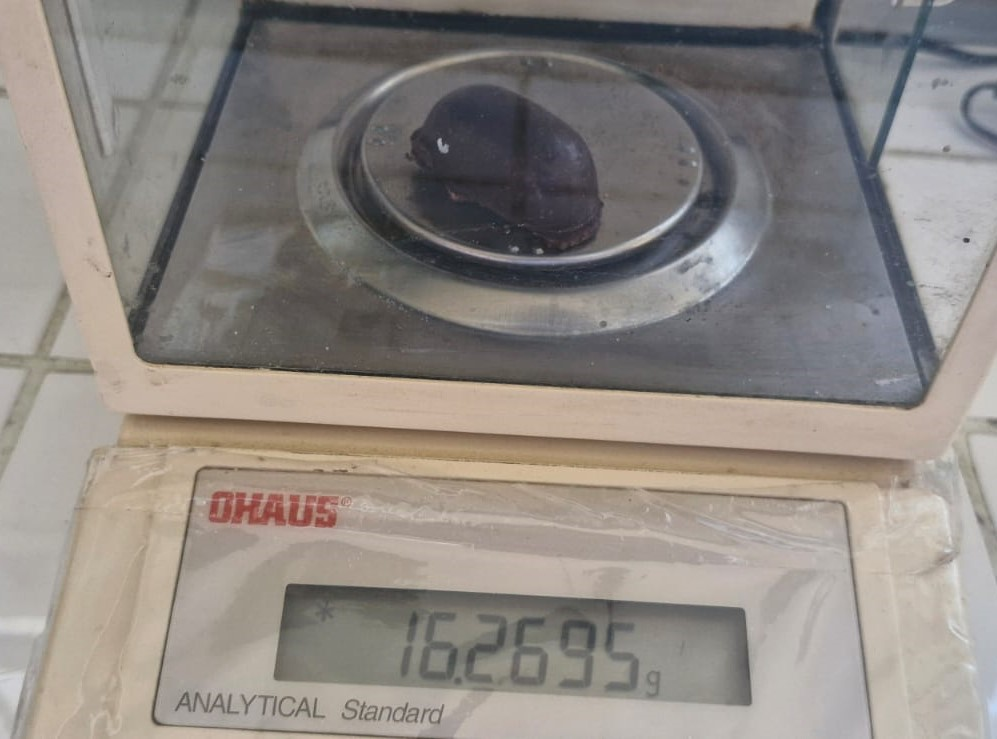
\includegraphics[width=\linewidth]{imagen/densidad 1.jpeg}
    \Description{Pesaje individual de chocoteja}
    \small (a) Pesaje de la chocoteja individual en balanza analítica (16.27 g).
  \end{minipage}
  \hspace{1em}
  \begin{minipage}{0.2\linewidth}
    \centering
    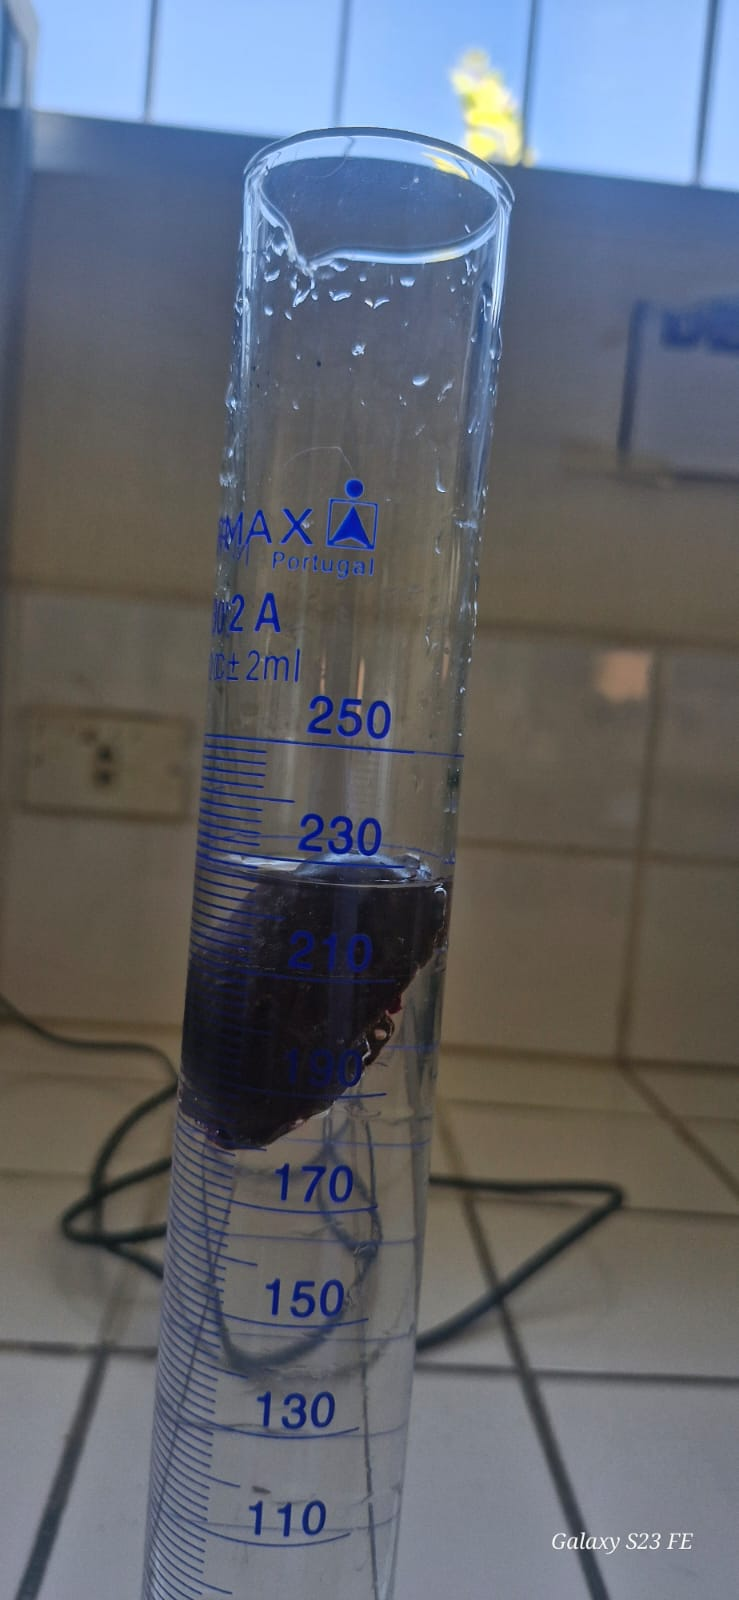
\includegraphics[width=\linewidth]{imagen/densidad.jpeg}
    \Description{Medición de volumen en probeta}
    \small (b) Medición de volumen desplazado en probeta para cálculo de densidad.
  \end{minipage}

  \vspace{1ex}
  % Segunda fila
  \begin{minipage}{0.3\linewidth}
    \centering
    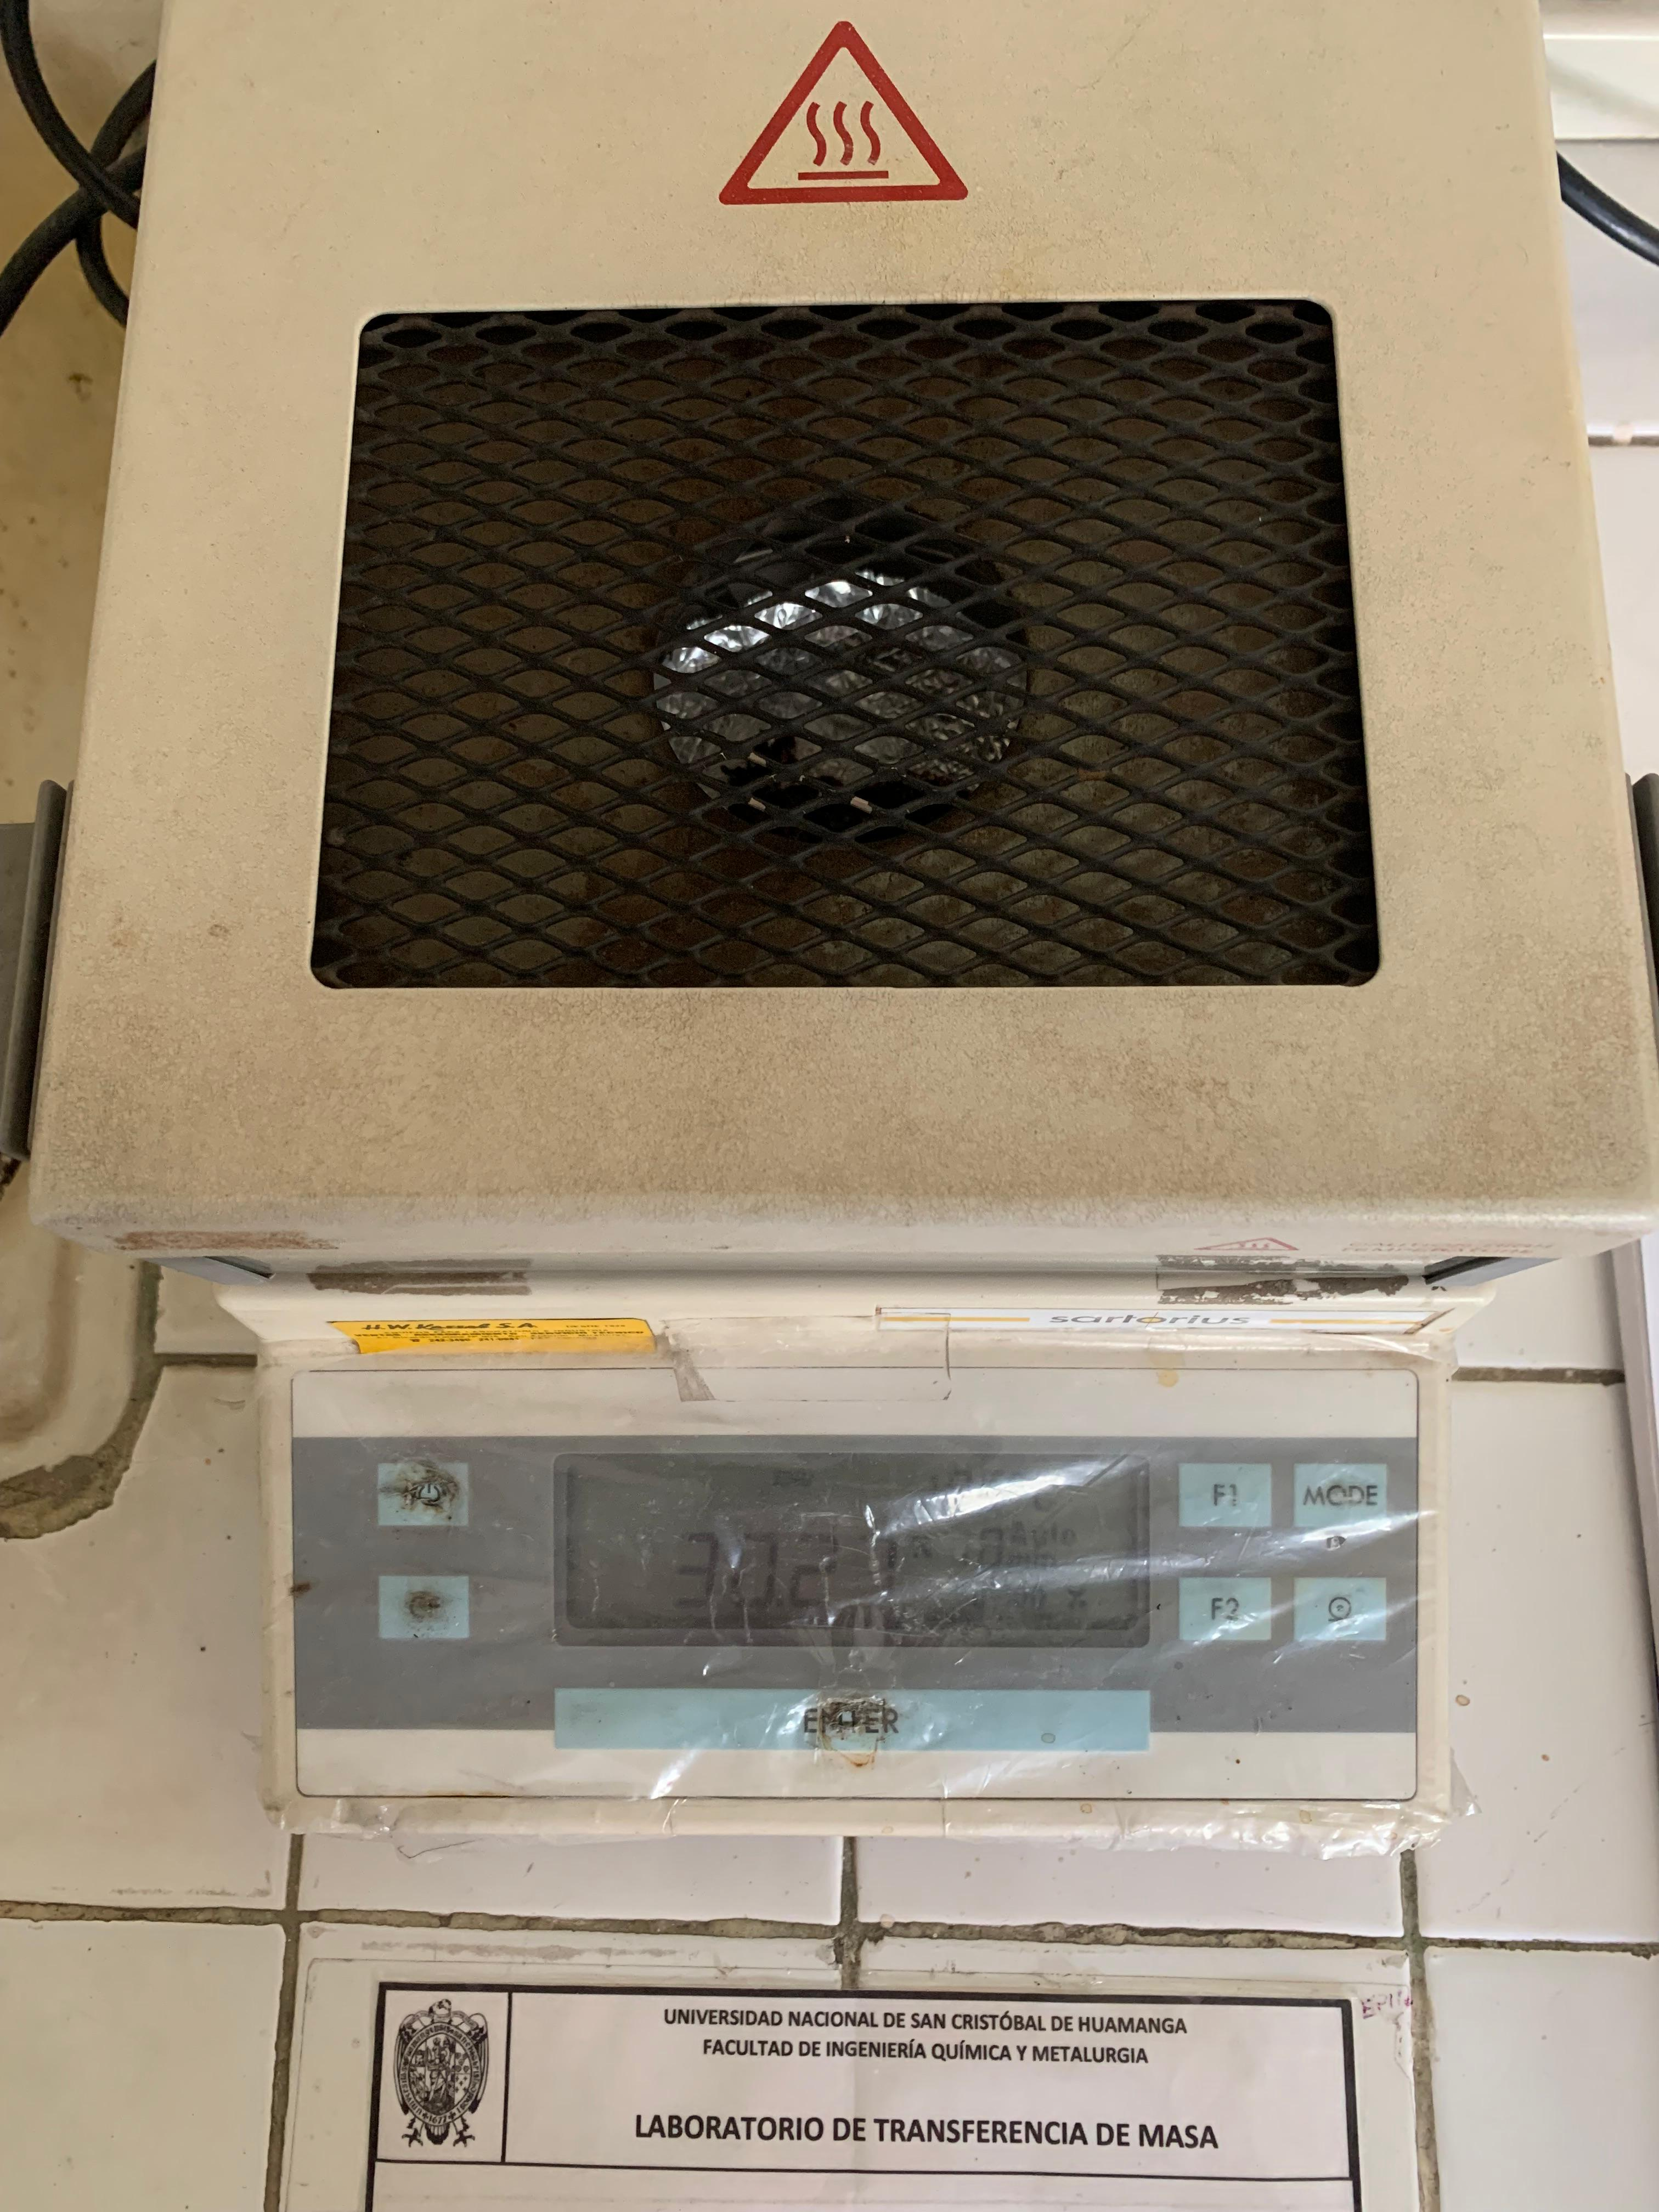
\includegraphics[width=\linewidth]{imagen/Humedad.jpeg}
    \Description{Determinación instrumental de humedad}
    \small (c) Determinación de humedad en balanza termogravimétrica.
  \end{minipage}
  \hspace{1em}
  \begin{minipage}{0.2\linewidth}
    \centering
    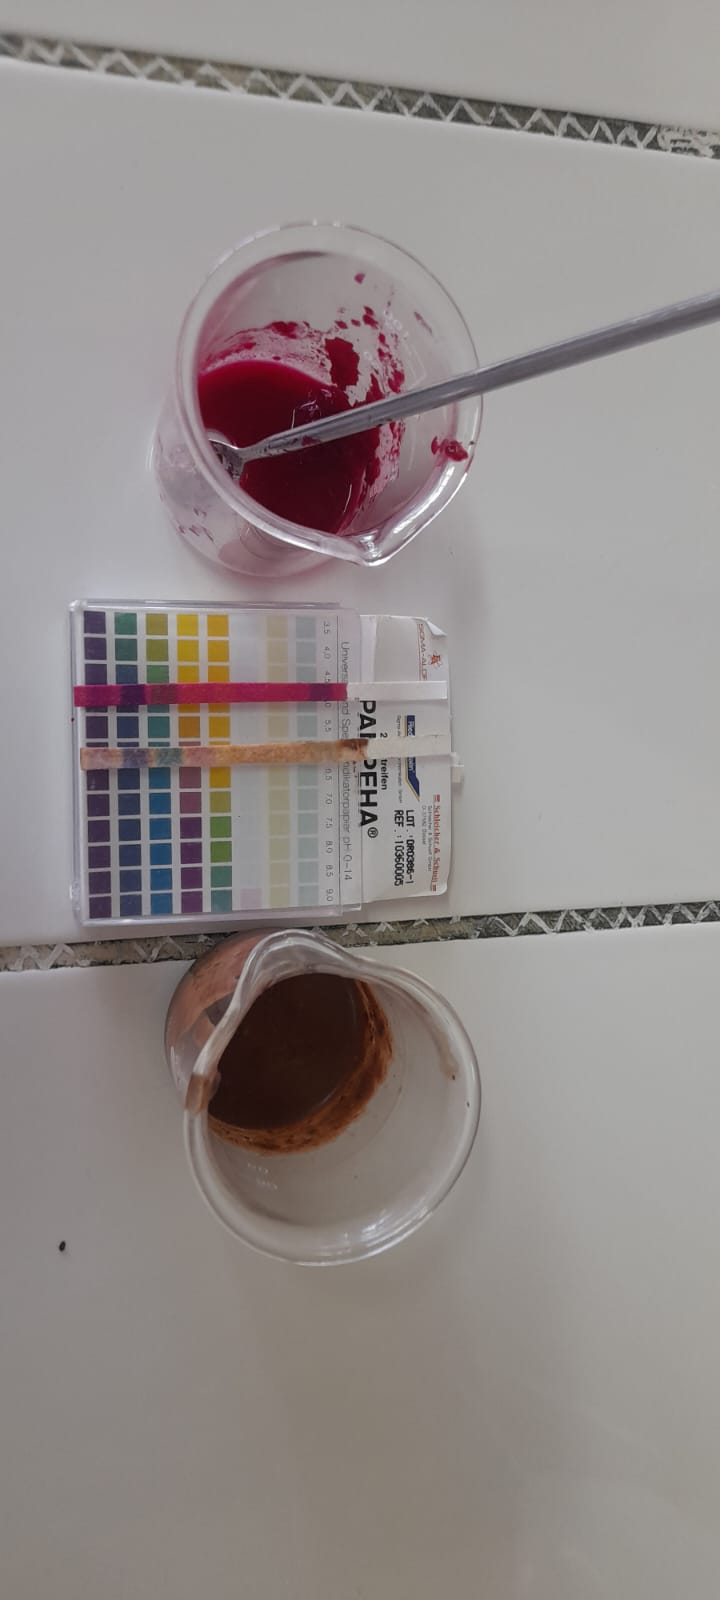
\includegraphics[width=\linewidth]{imagen/pH.jpeg}
    \Description{Evaluación de pH con tiras indicadoras}
    \small (d) Evaluación de pH mediante papel indicador.
  \end{minipage}

  \vspace{1ex}
  % Tercera fila
  \begin{minipage}{0.2\linewidth}
    \centering
    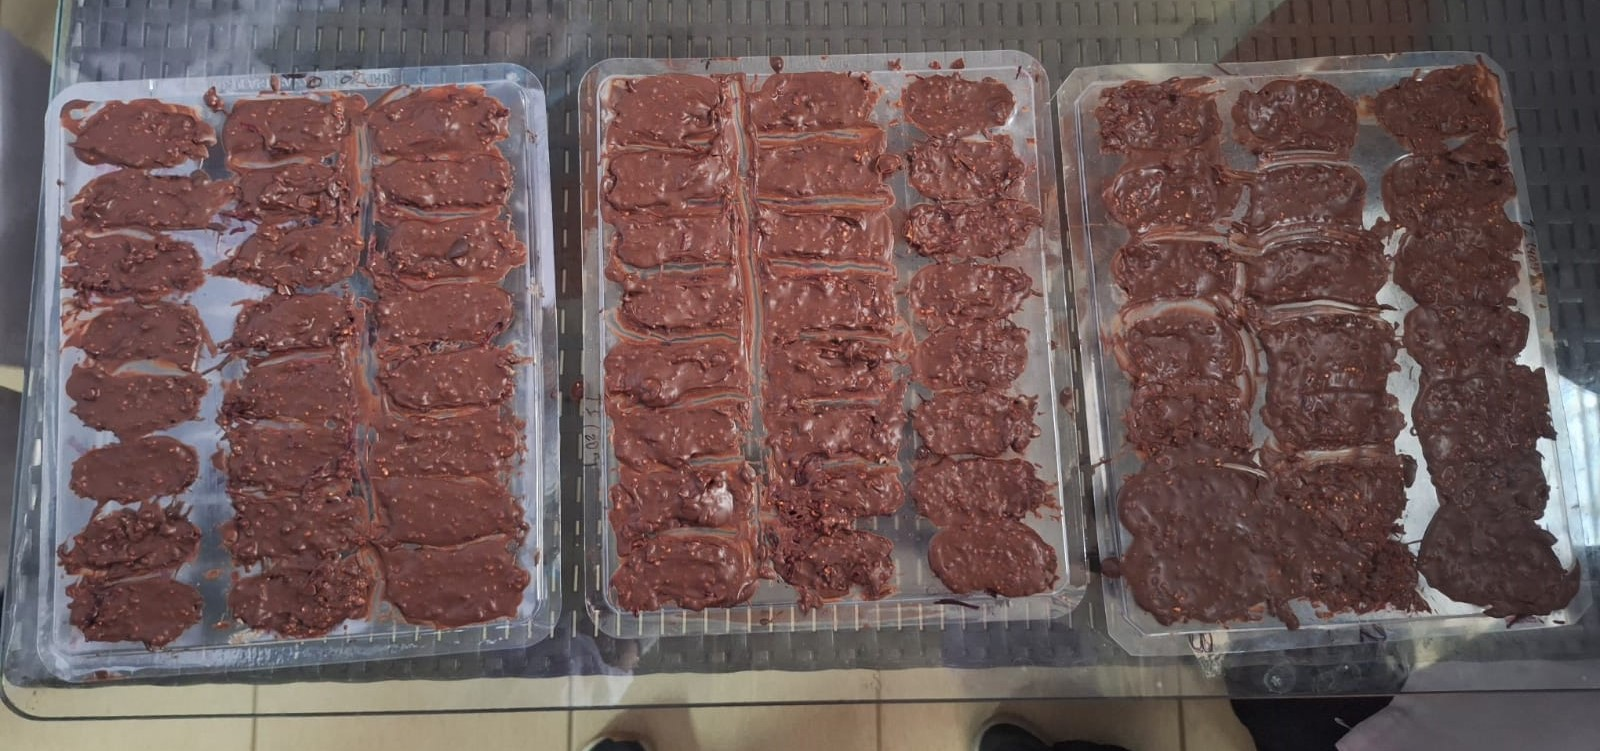
\includegraphics[width=\linewidth]{imagen/resultado 1.jpeg}
    \Description{Chocotejas terminadas en bandeja}
    \small (e) Chocotejas terminadas dispuestas en bandejas de moldeo.
  \end{minipage}

  \caption{Etapas del proceso de an\'alisis fisicoquímico y producción de chocotejas funcionales: determinación de densidad, humedad, pH y presentación final del producto.}
  \label{fig:proceso_analisis}
\end{figure}




%=========================================================

%=========================================================
\section{Discusión}
%=========================================================

Los resultados obtenidos confirman que el \emph{tiempo de cocción} es la variable que determina, en mayor medida, la calidad fisicoquímica y sensorial de las chocotejas elaboradas con beterraga, quinua y kiwicha \textit{pop}. El descenso significativo de la humedad y de la actividad de agua en los tratamientos cocidos (T\textsubscript{1} y T\textsubscript{2}) coincide con lo descrito por Arruda Ramos \textit{et al.}~\cite{ArrudaRamos2017}, quienes atribuían estas pérdidas a la gelatinización parcial del almidón y a la disrupción de estructuras celulares durante la cocción de la remolacha. Mantener $a_\mathrm{w}$ por debajo de 0.80 —y concretamente en torno a 0.77 en T\textsubscript{1}— implica una reducción sustancial del riesgo microbiológico y, por tanto, un potencial aumento de la vida útil sin añadir conservantes químicos.

En cuanto a la densidad aparente, el valor máximo registrado en el tratamiento intermedio (955~kg\,m$^{-3}$) sugiere una compactación óptima de la matriz debida a la redistribución de la fase gas–sólido durante la cocción. Este comportamiento respalda los planteamientos de Repo-Carrasco-Valencia y Singh~\cite{RepoCarrascoValencia2009,Singh2023}, para quienes la expansión controlada de pseudocereales \textit{pop} es clave para lograr texturas ligeras y crujientes, siempre que la humedad residual sea la adecuada. La estabilidad del pH, situada entre 6.7 y 6.8 en la cobertura y 5.3–5.4 en el relleno, concuerda con lo señalado por Montoya \textit{et al.}~\cite{Montoya2011} como rango óptimo para preservar betalainas y evitar el reblandecimiento del chocolate.

Desde el punto de vista sensorial, el tratamiento de 20 minutos (T\textsubscript{1}) alcanzó la mayor aceptabilidad global (8.1 ± 0.4). Esta preferencia se explica por la combinación de una humedad reducida —que evita sensación de pegajosidad— y una densidad suficiente para generar crocancia, sin llegar a producir las notas terrosas observadas en la muestra sobrecocida (T\textsubscript{2}). En términos tecnológicos, la cocción de 20 minutos permite suprimir etapas adicionales de secado, simplifica la línea de producción y reduce costos energéticos. Además, el producto resultante encaja con la tendencia de formulaciones \emph{clean label}, al lograr estabilidad con menor uso de aditivos. Todo ello, sumado al valor nutricional y la procedencia local de la quinua y la kiwicha, refuerza el potencial comercial de estas chocotejas como confitería premium de origen andino.

Aunque los datos son prometedores, el estudio se centró en la caracterización inicial; no se abordó la evolución de compuestos bioactivos ni la vida útil en condiciones comerciales. Futuros trabajos deberían cuantificar la estabilidad de betalainas y nitratos durante el almacenamiento, validar la inocuidad en escenarios de distribución reales y evaluar la huella ambiental del proceso para consolidar su perfil de sostenibilidad.

%=========================================================
\section{Conclusiones}
%=========================================================

El tratamiento térmico de 20 minutos se identifica como la condición óptima para fabricar chocotejas con beterraga, quinua y kiwicha \textit{pop}. Bajo este tiempo de cocción se logró la menor actividad de agua ($a_\mathrm{w}\leq 0.77$), una densidad aparente de 955 kg\,m$^{-3}$ asociada a una textura crujiente y la máxima aceptación sensorial registrada. Los tiempos extremos evaluados alteraron la calidad: la muestra cruda retuvo demasiada humedad y perdió crocancia, mientras que la muestra de 40 minutos desarrolló notas terrosas y un relleno ligeramente deshidratado.

Desde la perspectiva industrial, la cocción intermedia reduce el consumo energético —al prescindir de secados adicionales— y facilita la obtención de productos con etiquetado \emph{clean label}. Además, integra ingredientes andinos de alto valor añadido, fortaleciendo cadenas agrícolas locales y atendiendo la demanda de snacks vegetales con perfil saludable.

El presente estudio se limita a la evaluación inmediata; no se cuantificaron compuestos bioactivos ni se estudió la vida útil prolongada. En consecuencia, se recomienda investigar la estabilidad de betalainas y nitratos a lo largo del almacenamiento, realizar ensayos de vida útil en condiciones de mercado y cuantificar la huella de carbono del proceso. Estas acciones permitirían consolidar la propuesta como una confitería diferenciada, sostenible y de alto potencial comercial.
































%%%%%%%%%%%%%%%%%%%%%%%
%%%%%%%%%%%%%%%%%%%%%
%%%%%%%%%%%%%%%%%%%%%%
% Restore sectioning commands
\makeatletter
\let\section\ACM@origsection
\let\subsection\ACM@origsubsection
\let\subsubsection\ACM@origsubsubsection
\makeatother
\bibliographystyle{ACM-Reference-Format}
\bibliography{sample-base}
\end{document}
